\section{Travaux effectués} 

\subsection{\Gls{classification} des images par qualité, face profils}
L'objectif fixé à la première visio conférence a été déterminé : faire de la \gls{classification} sur la qualité des photographies des mandrills.\\

J'ai donc commencé par faire du \gls{transfer learning} avec MobileNet V2, un réseau neuronal convolutif (CNN)  de Google adapté aux mobiles (c'est-à-dire, très rapide et plutôt performant) pour essayer d'adapter un modèle avec les poids ImageNet pour la \gls{classification} de la qualité des photographies. Notre \gls{dataset} ressemble aux images ci-dessous, avec FaceQual0-3 en label de qualité, 3 étant la meilleure qualité.

\begin{figure}
    \centering
    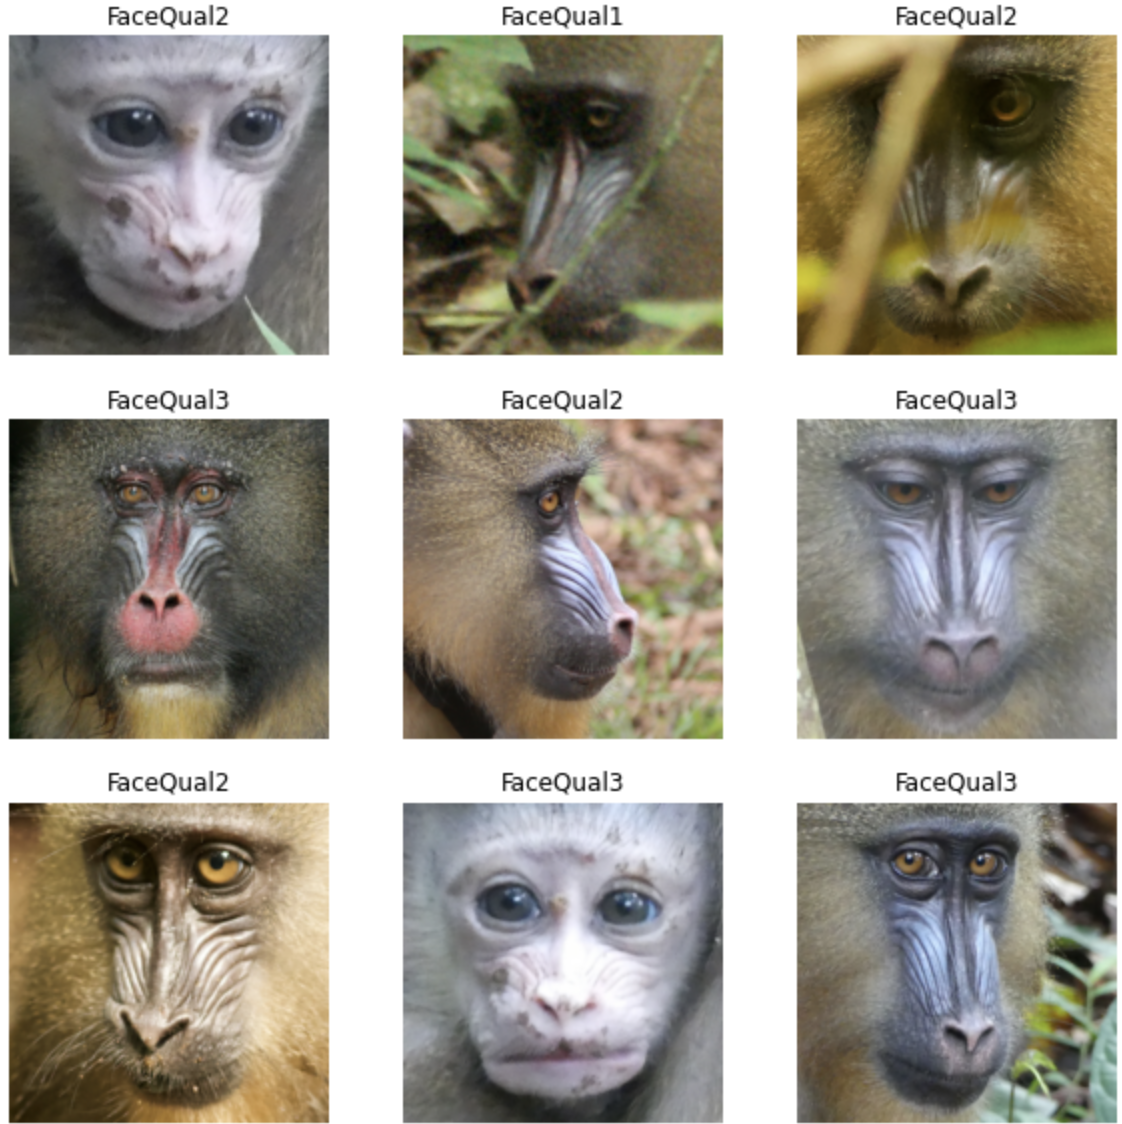
\includegraphics[width=300pt]{imgs/qualité/cr1/dataset.png}
    \caption{Exemples d'images avec leur label qualité correspondant}
    \label{fig:my_label}
\end{figure}

Les premiers résultats semblent bons à première vue : 85\% d'\gls{accuracy} sur une \gls{classification} simple.

\begin{figure}
    \centering
    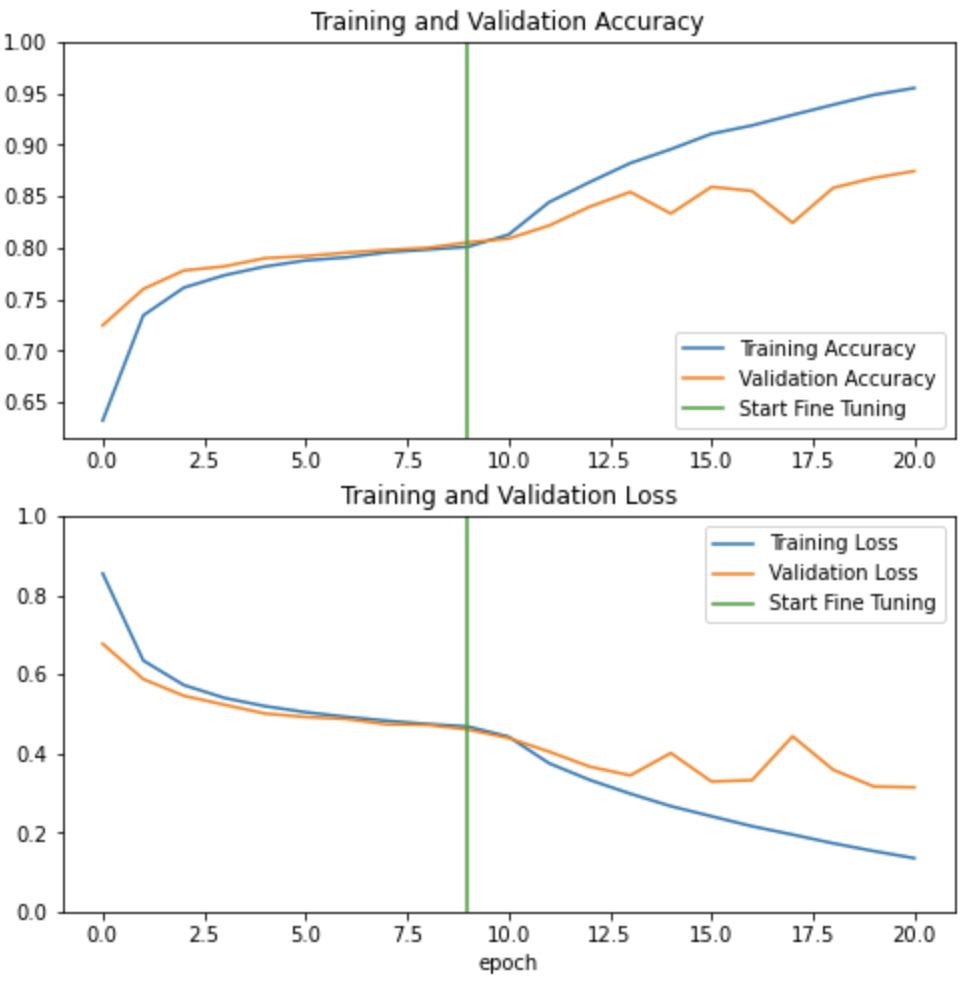
\includegraphics[width=300pt]{imgs/qualité/cr1/resultat1.png}
    \caption{Résultat}
    \label{fig:my_label}
\end{figure}

\begin{figure}
    \centering
    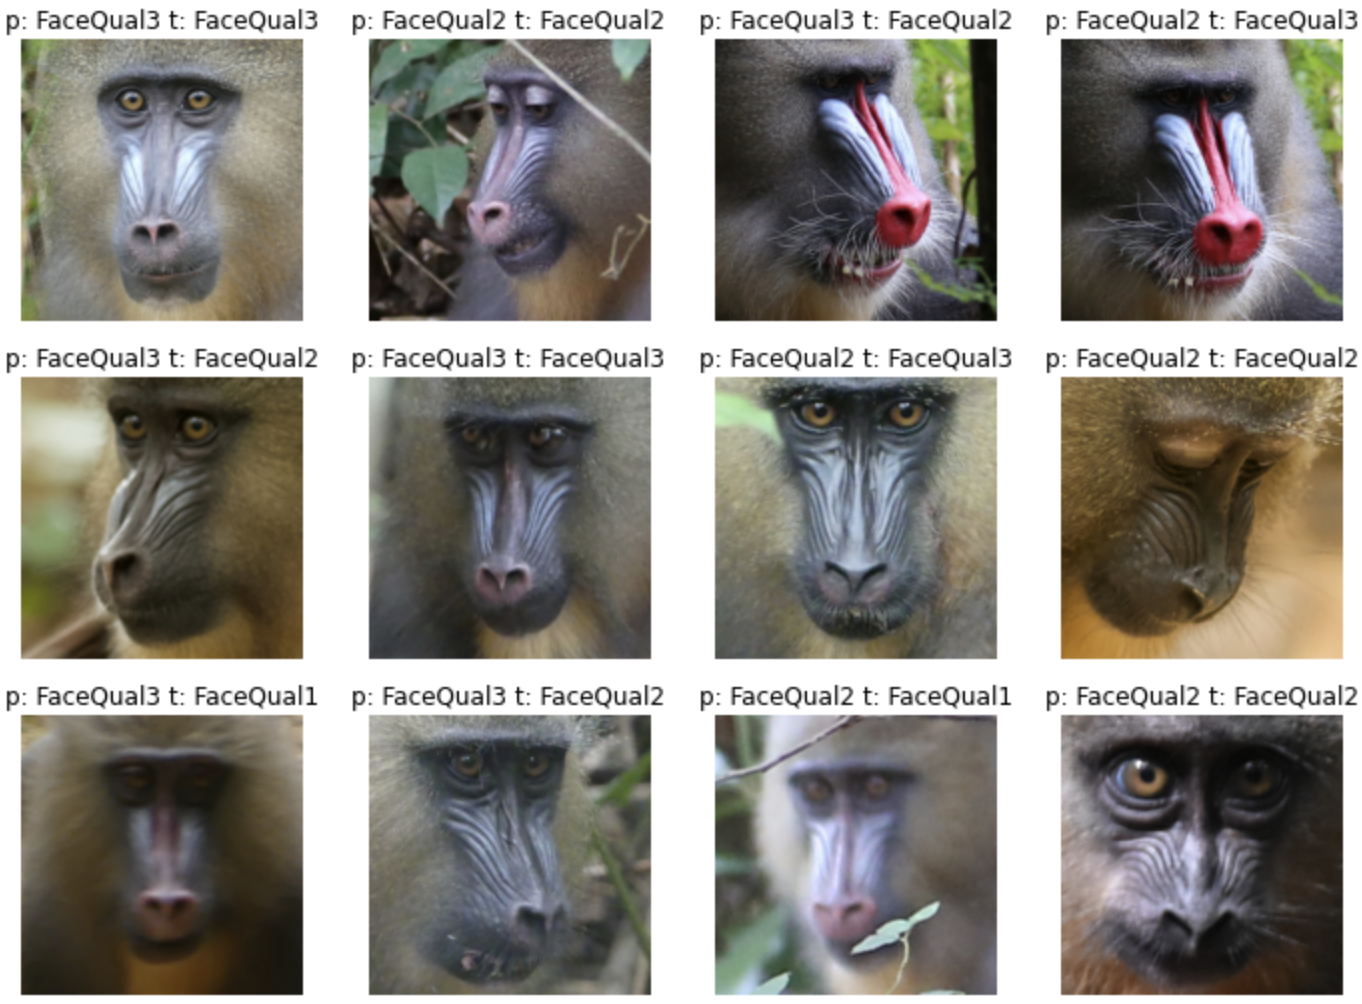
\includegraphics[width=300pt]{imgs/qualité/cr1/prediction1.png}
    \caption{Prédictions}
    \label{fig:my_label}
\end{figure}

Mais les résultats sont trompeurs, en effet, le jeu de données est très déséquilibré, avec 10000 images de qualité FaceQual2 et 6000 de qualité FaceQual3 contre 250 et 1000 de qualité FaceQual0 et FaceQual1. Le modèle pourrait donc prédire tout le temps FaceQual2 et avoir 57\% d'\gls{accuracy} par défaut.\\

Il faut donc gérer ce déséquilibre, et deux approches nous paraissent intéressantes :\\
\begin{itemize}
    \item dégrader des images de bonne qualité (downscale puis upscale et léger floutage) pour génerer des photos de mauvaises qualité (une mauvaise photo souvent a un manque de détails et/ou est flou).
    \item pondérer les classes de jeu de données pendant l'entrainement (accorder plus d'importance donc là où on aurait moins d'échantillons).
\end{itemize}

Voici un exemple de ce que pourrait être une dégradation d'images par rapport aux premières images :

\begin{figure}
    \centering
    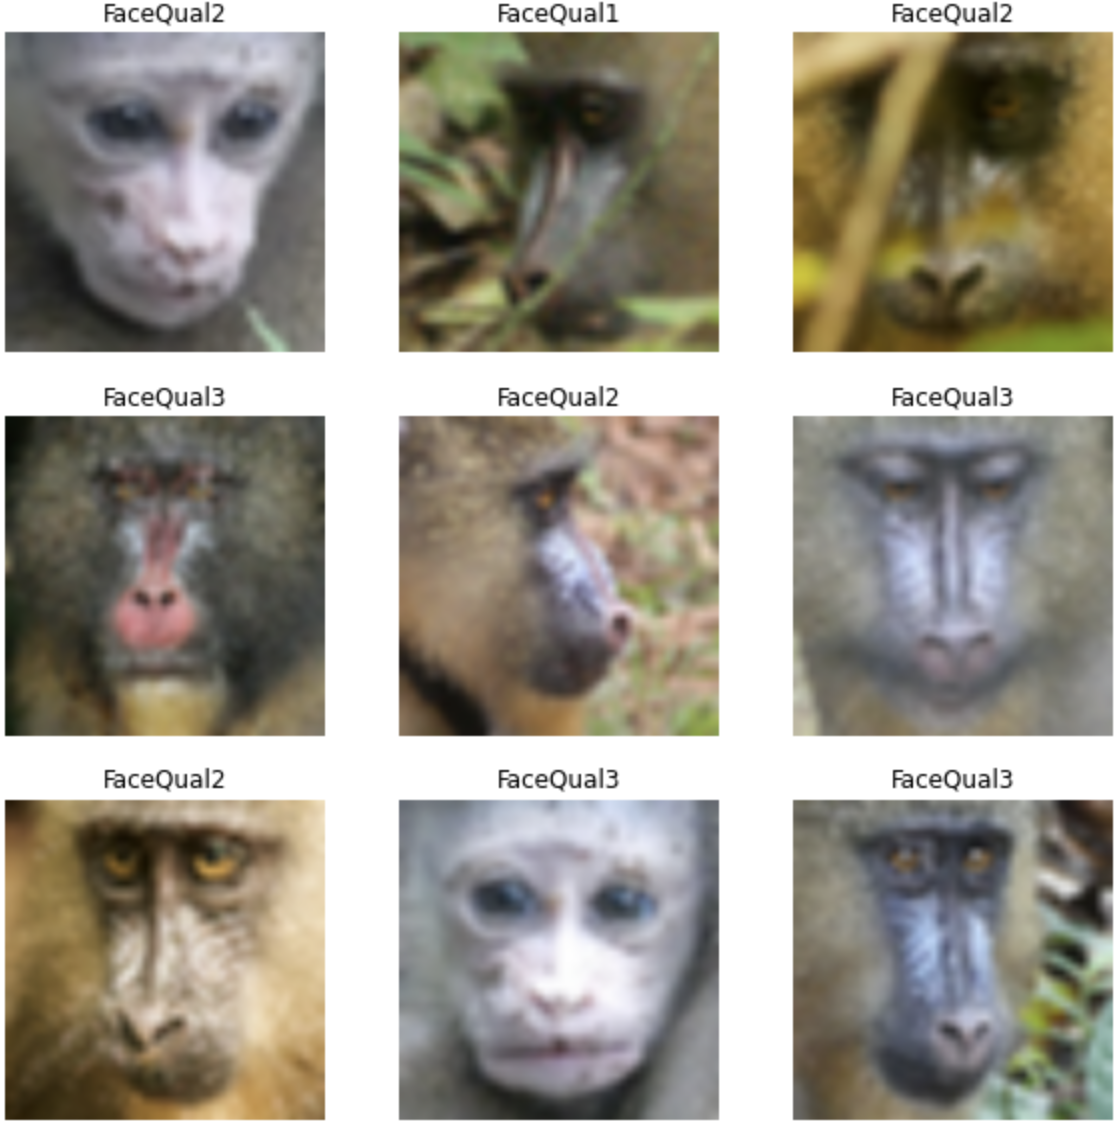
\includegraphics[width=300pt]{imgs/qualité/cr1/augmentation1.png}
    \caption[Images dégradées]{Voici les mêmes images que sur la figure 1, mais avec une opération de dégradation par floutage et downscale/upscale. On peut voir qu'une photo de bonne qualité normalement ne l'est plus.}
    \label{fig:my_label}
\end{figure}

\begin{figure}
    \centering
    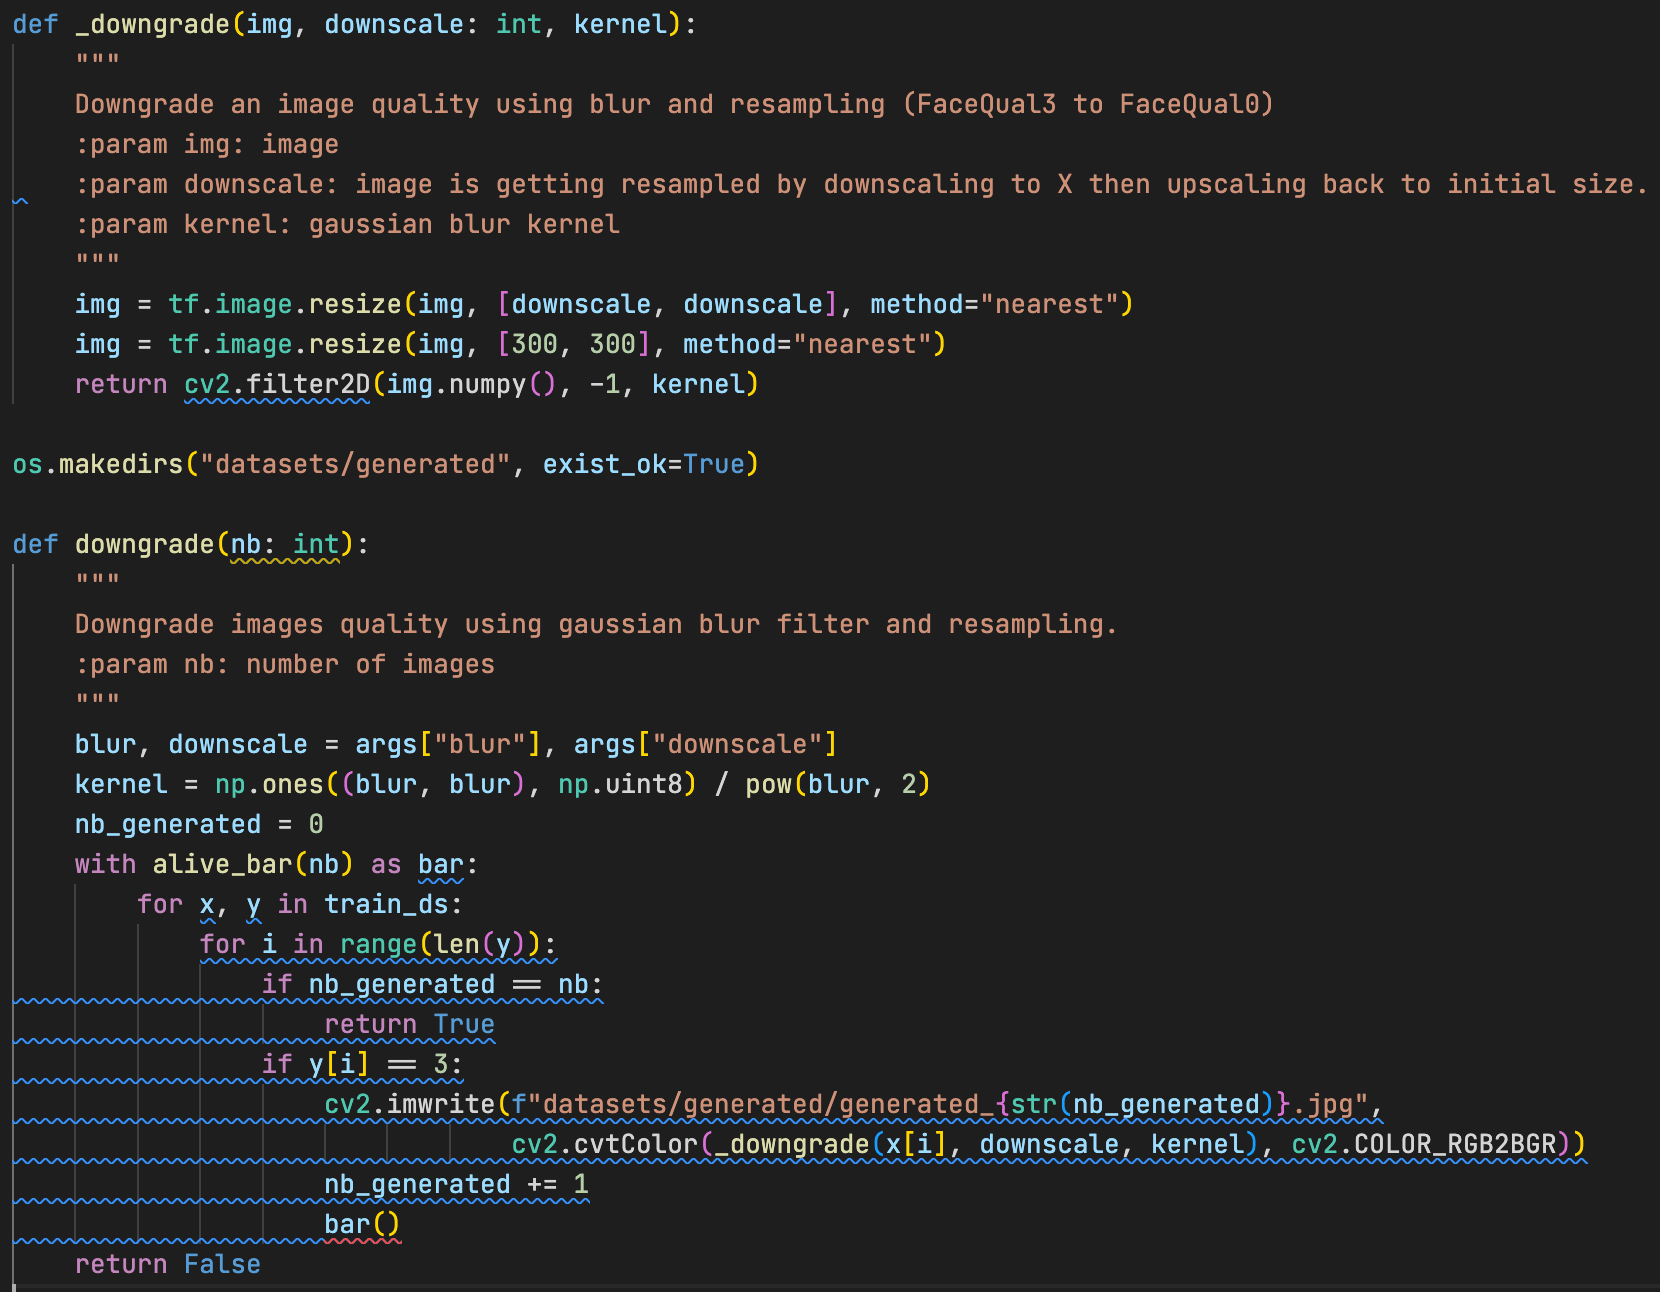
\includegraphics[width=300pt]{imgs/qualité/cr9/generate.png}
    \caption[Code pour dégrader les images]{Fonctions permettant de générer les images de qualité mauvaises (0) à partir des images de très bonne qualités (3). Le but étant de réduire l'impact de l'imbalance des classes, on créé autant d'images de qualité 0 qu'il n'en faut pour égaliser la classe 0 et la classe 1.}
    \label{fig:my_label}
\end{figure}

Évidemment, on peut faire varier le niveau de floutage et de dégradation de détails. On pourrait également imaginer appliquer un fort taux de compression JPEG ou augmenter le bruit artificiellement pour obtenir des images de basse qualité réalistes (tout cela étant des facteurs de basse qualité).\\

Ensuite, j'ai travaillé sur la \gls{matrice de confusion} et le \gls{graphe ROC} et commencer à comparer de manière plus complète les modèles.\\

Nous démarrons avec un \gls{transfer learning} par VGG16/ImageNet suivi de deux couches complètement connectés, de type Dense (chaque neurone, de chaque couche, est inter connecté) et avec une activation \gls{ReLU} (non linéaire), et par enfin une couche de type Dense avec une activation SoftMax (probabilités, entre 0 et 1).

Nous obtenons sur 10 epochs un rappel à 0.8 pour les 2 classes les plus représentés (FaceQual2/3) et 0.65 pour les autres (FaceQual0/1). Cela veut donc dire qu'une proportion correcte initiale d'échantillons est correctement classé.

\begin{figure}
    \centering
    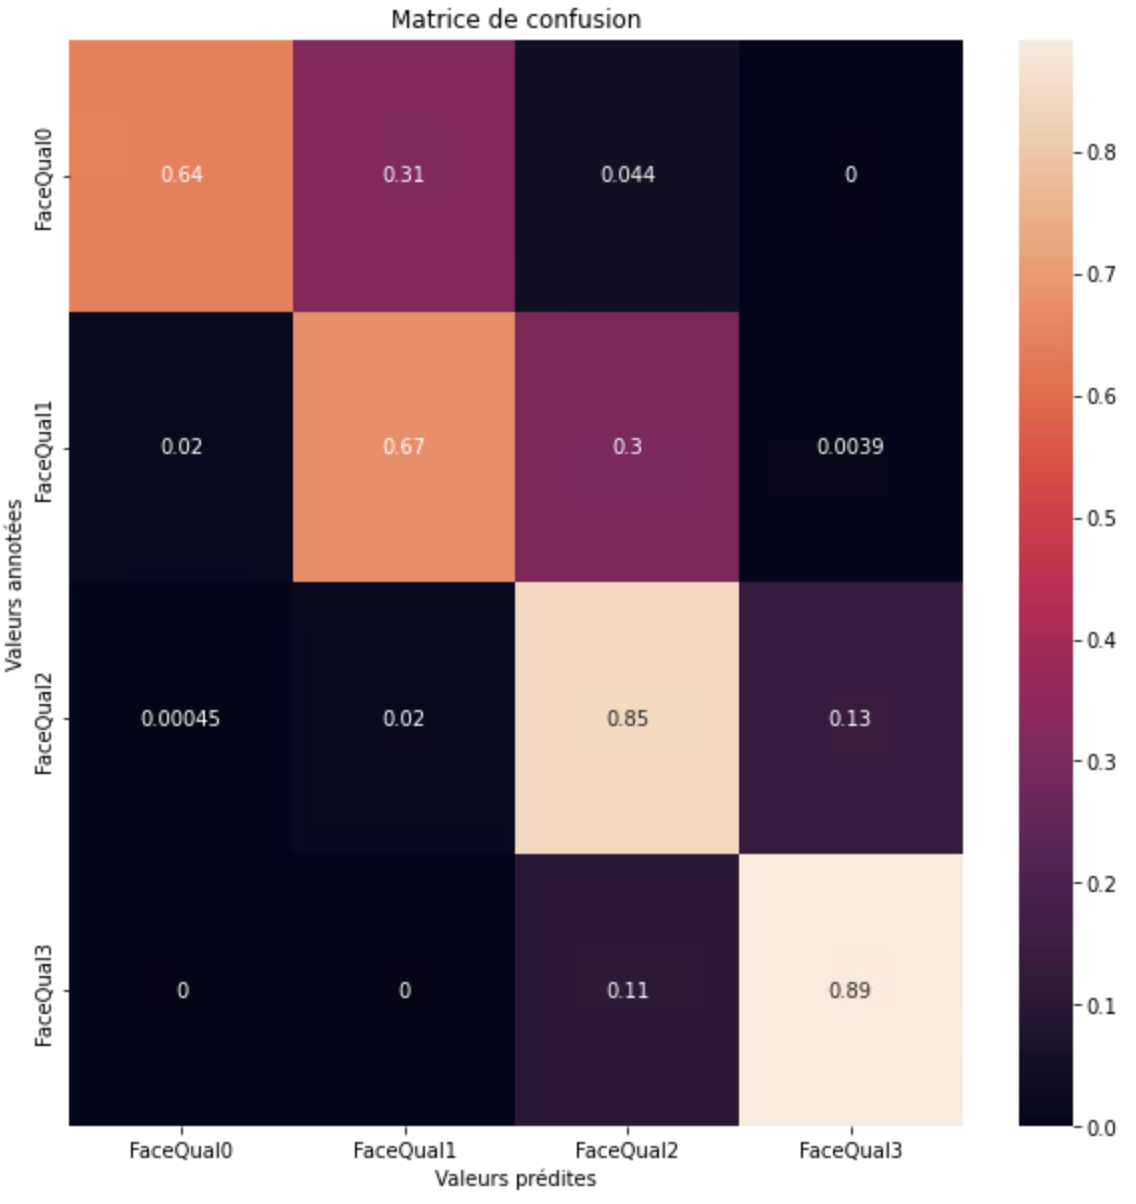
\includegraphics[width=300pt]{imgs/qualité/cr2/vgg16_000_confusion.png}
    \caption[Matrice de confusion pour une 1re classification]{\Gls{Matrice de confusion} représentant le taux d'échantillons prédis par classe pour chacuns des labels connus. Par exemple, 64\% des échantillons FaceQual0 ont correctement été prédis, et 31\% ont été prédis avec une classe d'écart (FaceQual1).}
    \label{fig:my_label}
\end{figure}

\begin{figure}
    \centering
    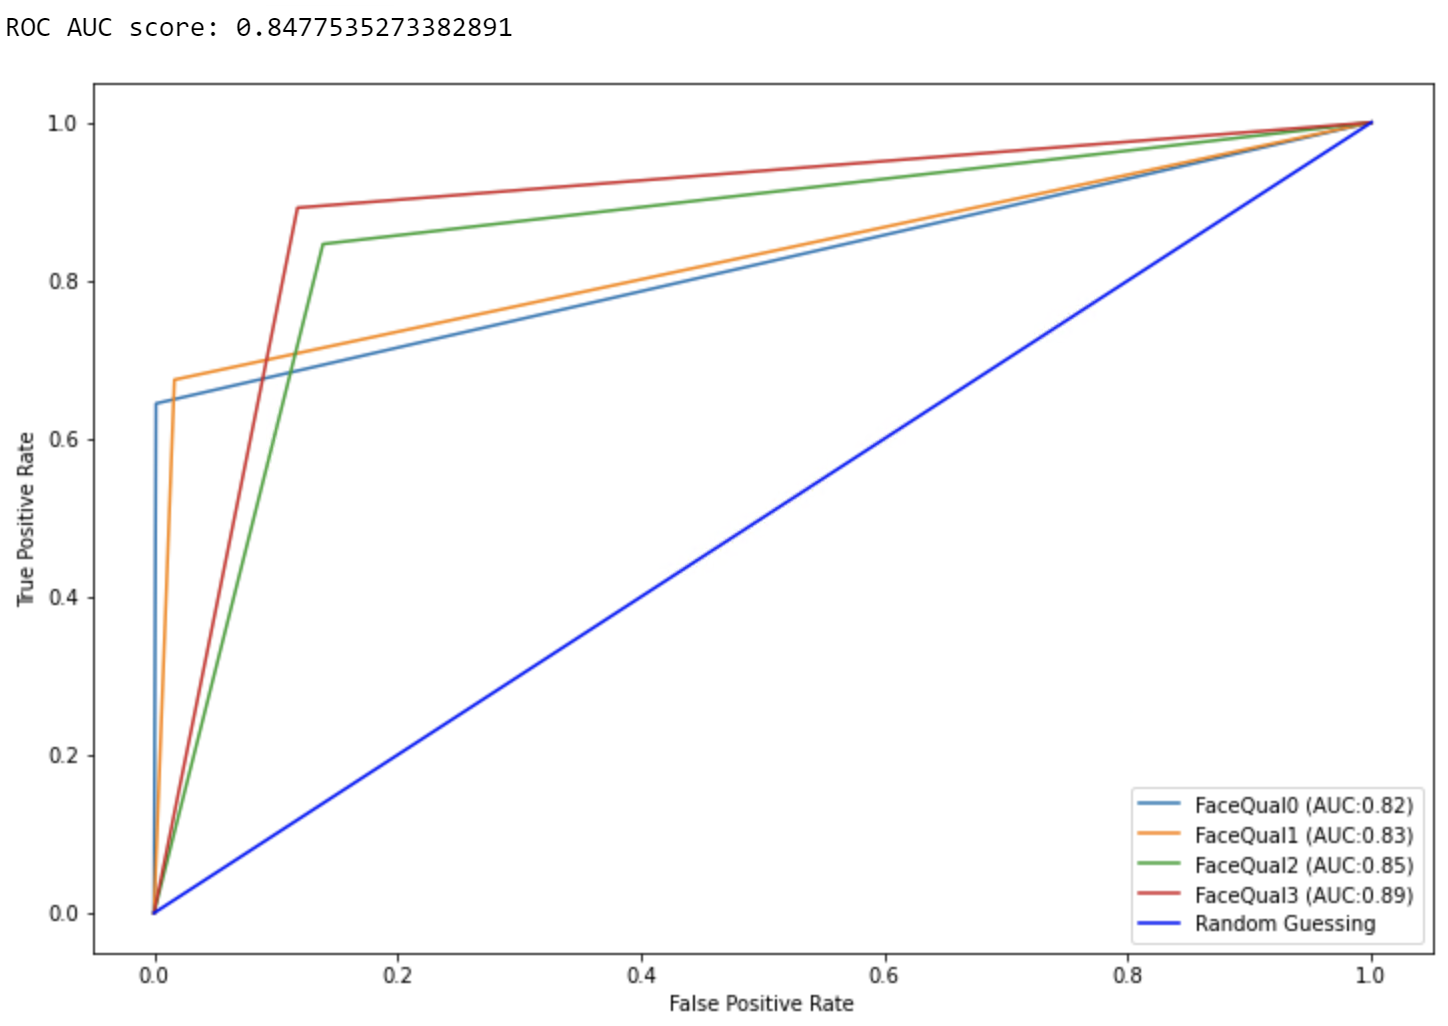
\includegraphics[width=300pt]{imgs/qualité/cr2/vgg16_000_roc.png}
    \caption[Courbe ROC associé pour une 1re classification]{La \gls{courbe ROC} montre que les classes avec un plus faible taux de vrais positifs (les images de mauvaises qualités) ont également un taux plus faible de faux positifs. Cela veut dire qu'il est rare qu'une image de bonne qualité soit considéré comme de mauvaise qualité, mais qu'il arrive qu'une image de mauvaise qualité soit considéré de bonne qualité.}
    \label{fig:my_label}
\end{figure}

Pour améliorer la situation, problématique sûrement à cause du déséquilibre des données, nous pouvons essayer d'abord la pondération des classes. Cela permet en effet d'améliorer largement le résultat de la classe la plus sous représentée (FaceQual0), avec un poids d'importance de 17. Seulement, une partie de l'apprentissage est troublée, d'une part car la classe FaceQual1 est partiellement confondue par la classe FaceQual0 et également du fait que beaucoup d'échantillons FaceQual2 sont classés en FaceQual0 (5\% des FaceQual2, représentant une bonne partie sachant que FaceQual2 possède énormément plus d'images).


\begin{center}
    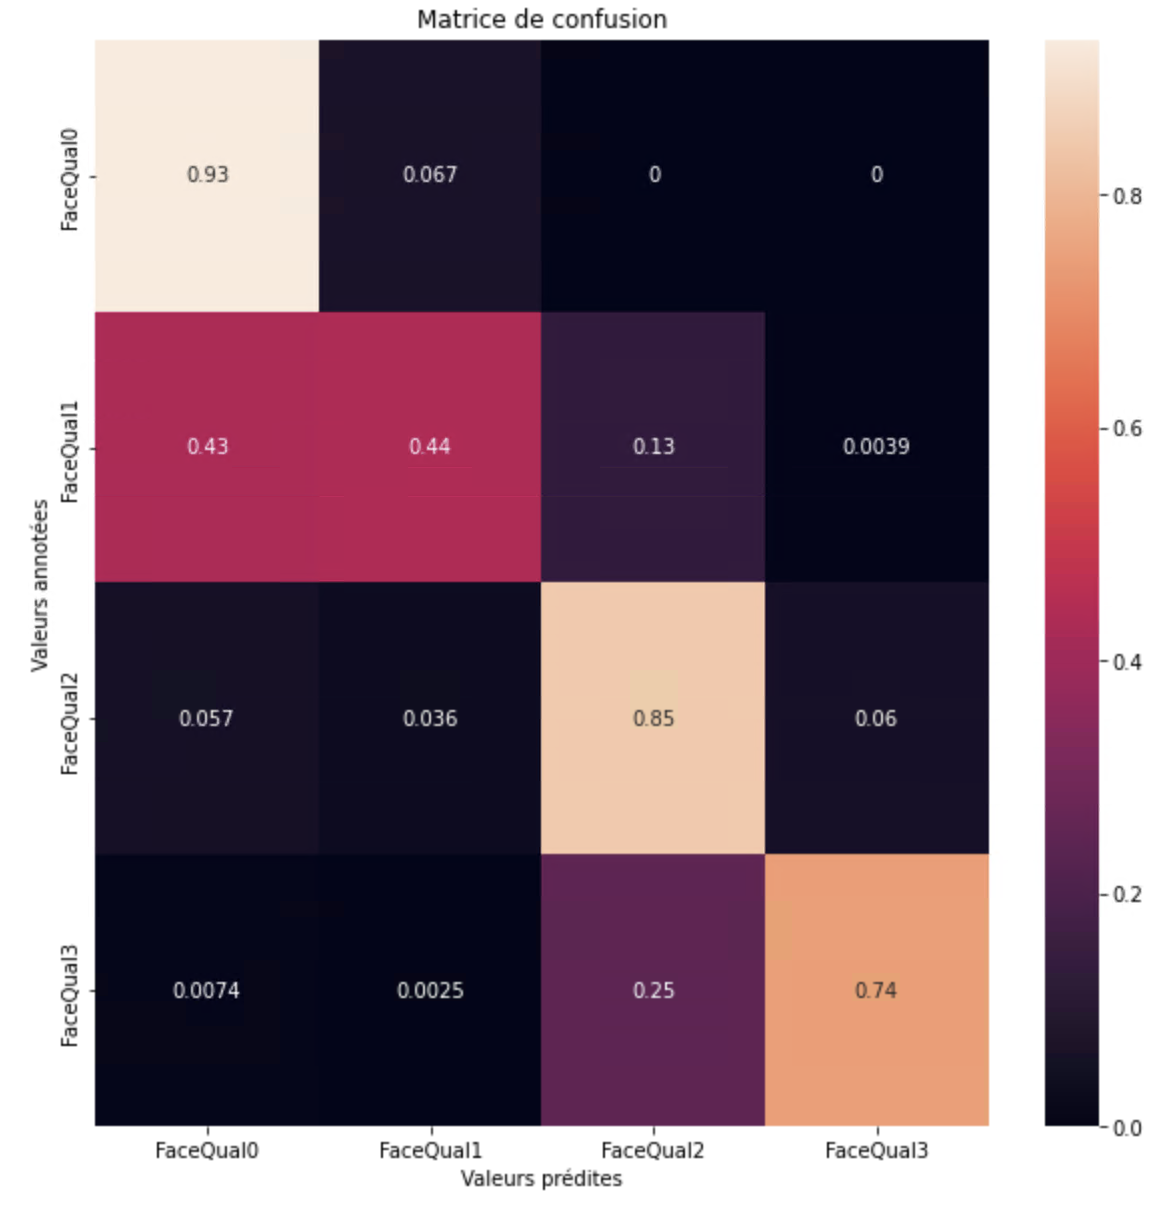
\includegraphics[width=210pt]{imgs/qualité/cr2/vgg16_010_confusion.png}
    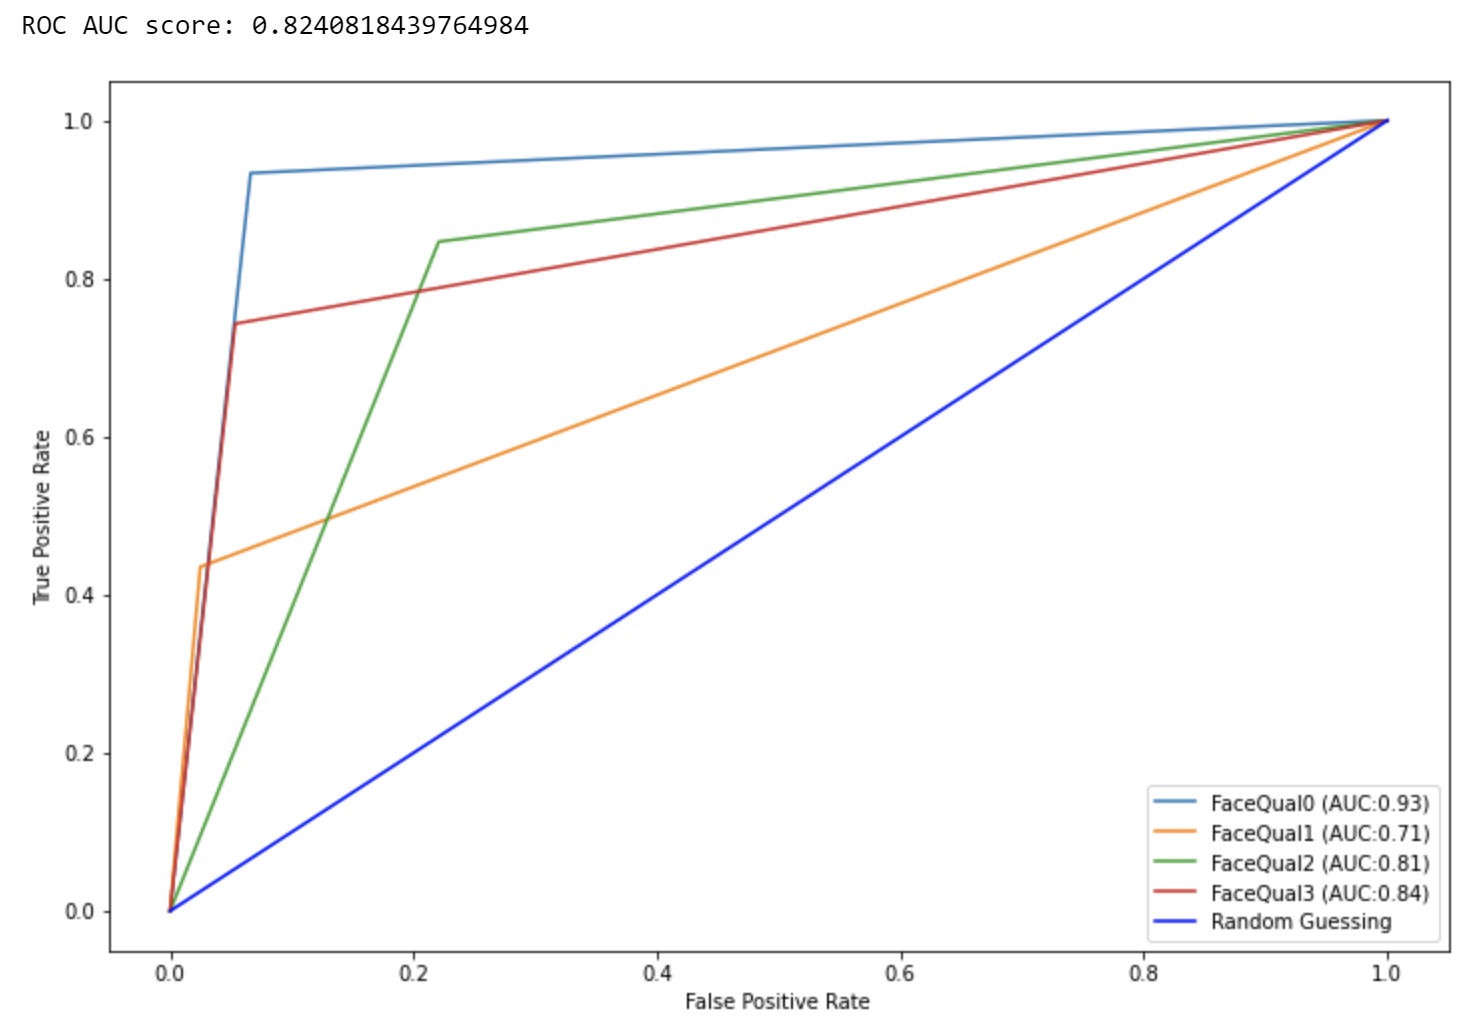
\includegraphics[width=210pt]{imgs/qualité/cr2/vgg16_010_roc.png}
\end{center}

Une piste est alors d'opérer un \gls{oversampling} a priori sur la classe FaceQual0 pour avoir des poids de classes plus adéquats (moins grands). \\

Une fois testé, nous trouvons un \gls{rappel} supérieur à la situation initiale sans cette fois-ci occasionner de dommages collatéraux. Le poids de la classe FaceQual0 après l'\gls{oversampling} par copie/dégradation des images FaceQual3 est autour de 4, soit 4 fois moins qu'avant \gls{oversampling}.

\begin{center}
    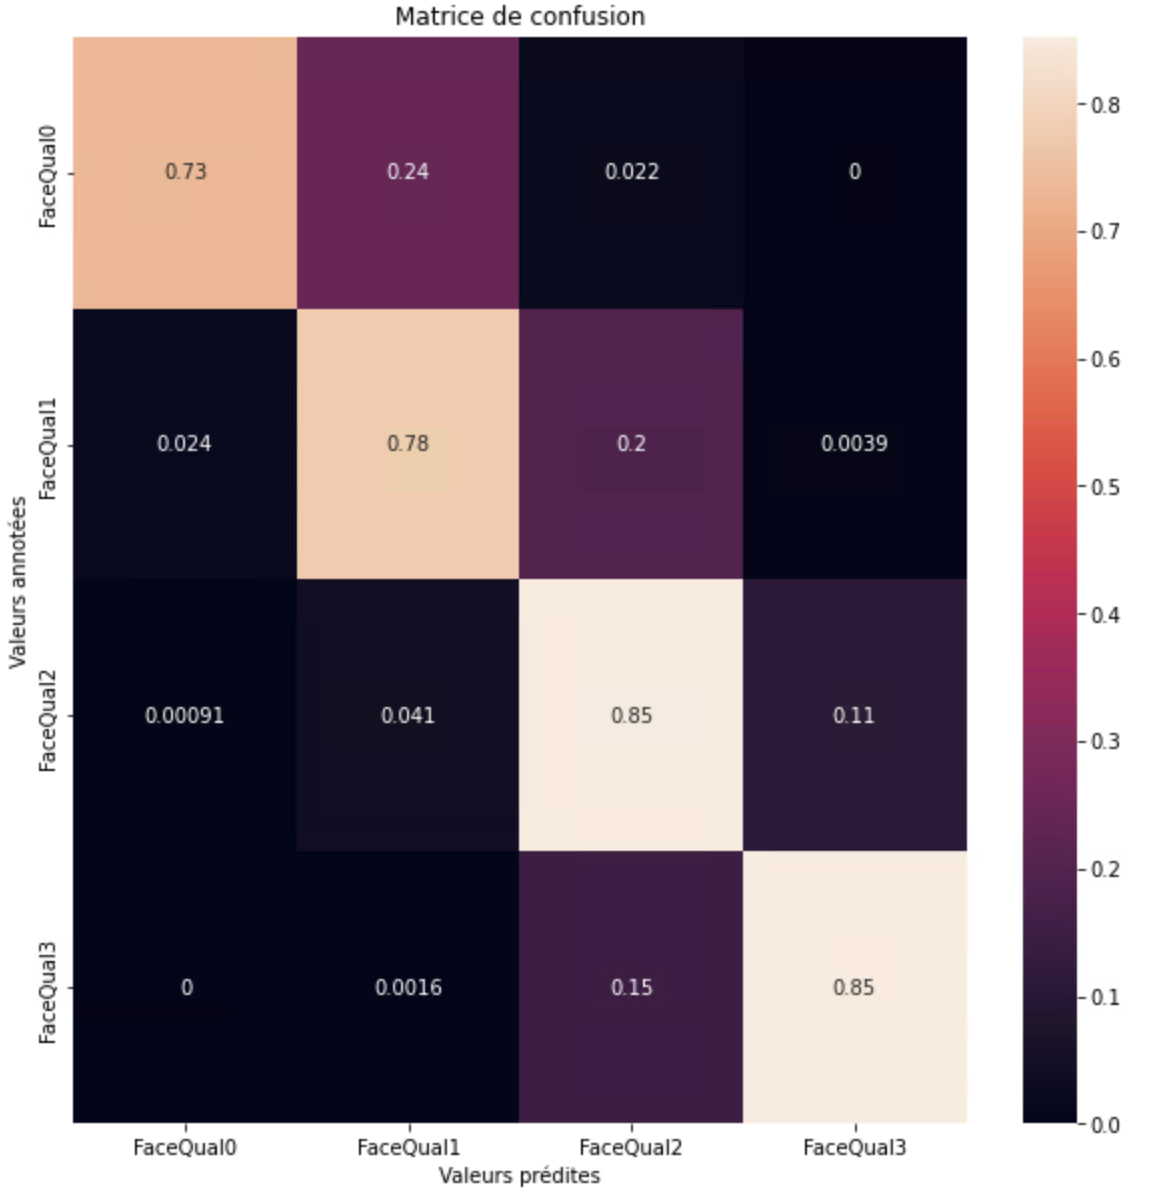
\includegraphics[width=210pt]{imgs/qualité/cr2/vgg16_011_confusion.png}
    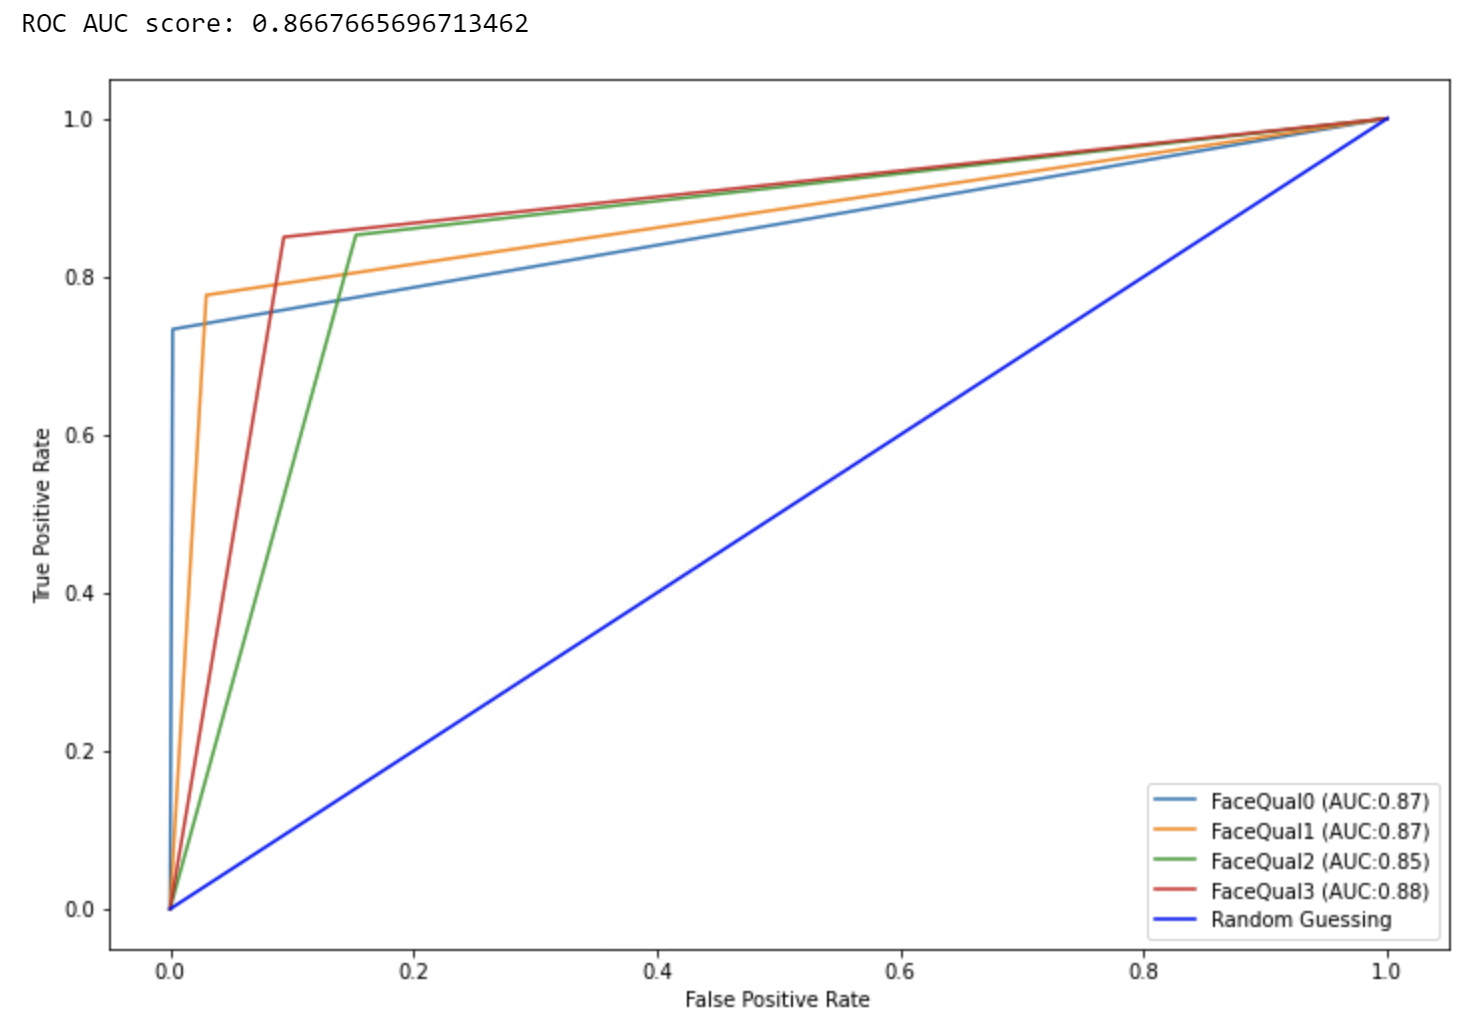
\includegraphics[width=210pt]{imgs/qualité/cr2/vgg16_011_roc.png}
\end{center}

\subsection{Prédictions de classes ordonnées}
Pour résoudre ce problème de \gls{classification}, il est tentant de réduire le problème à une régression, puisque les classes sont corrélés : les classes 1FaceQual0-3 correspondent à une suite d'images de qualité croissante.
Enfin, pour les classifier de manière discrète, il suffirait d'arrondir les prédictions alors continus.
\begin{center}
    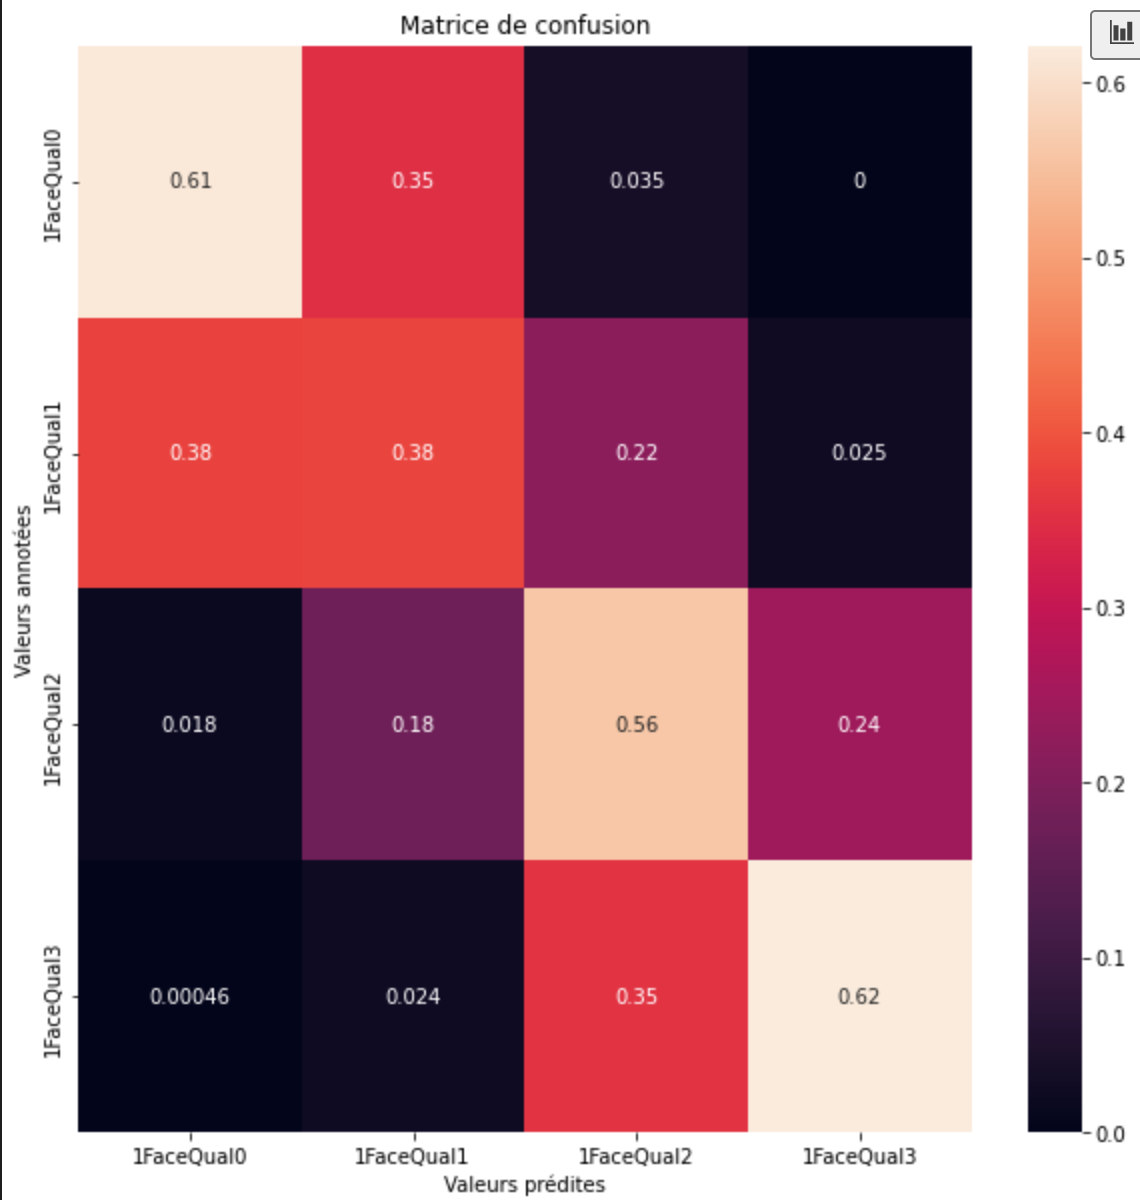
\includegraphics[width=300pt]{imgs/qualité/cr6/confusion-regression.png}
\end{center}

Le résultat n'est cependant pas aussi bon. Cela est sûrement en partie dû au fait que les valeurs ne sont pas prédites dans l'intervalle [0; 3] mais $[-\infty; +\infty]$.

On peut supposer affiner les résultats en améliorant les méthodes liés à la normalisation, ou alors en retournant au modèle de \gls{classification} d'avant avec cross entropy.

Une autre méthode à explorer pour résoudre un problème de \gls{classification} multi classes ordonné, est d'utiliser un encodage one-hot particulier tel que décrit sur cette \href{https://stats.stackexchange.com/questions/140061/how-to-set-up-neural-network-to-output-ordinal-data}{réponse} et  \href{https://arxiv.org/pdf/1901.07884.pdf}{papier}.
J'ai donc créé un générateur personnalisé d'images, qui prend des \gls{batch} d'images avec leur label et retourne normalement les mêmes \gls{batch} avec les mêmes labels encodés sous la nouvelle forme :\\
\begin{gather*}
0 \longrightarrow [0, 0, 0]\ (au\ lieu\ de\ [1, 0, 0, 0])\\
1 \longrightarrow [1, 0, 0]\ (au\ lieu\ de\ [0, 1, 0, 0])\\
2 \longrightarrow [1, 1, 0]\ (au\ lieu\ de\ [0, 0, 1, 0])\\
3 \longrightarrow [1, 1, 1]\ (au\ lieu\ de\ [0, 0, 0, 1])\\
\end{gather*}
Par ailleurs, au lieu d'utiliser une dernière couche à k neurones et pour activation softmax, j'utilise k-1 neurones avec pour activation sigmoid. Enfin, pour avoir le numéro de la classe prédite, on fait la somme des probabilités, ce qui donne par exemple : $[1,1,0] \longrightarrow 2
[img onehot]$

\subsection{Base de données des métadonnées}
Avant le commencement du stage, les métadonnées étaient répartis sur plusieurs fichiers \gls{CSV}. Cela induisait donc une certaine dureté pour y appliquer des modifications, ainsi qu'une rigidité pour utiliser les fichiers.\\

Alors nous nous sommes poser la question s'il pourrait être intéressant de créer une base de données pour organiser mieux le lien entre les métadonnées d'une image originale, d'une image portrait, d'un individu mandrill, etc...
Pour moi, le choix le plus cohérent était de partir sur une base de données \gls{SQLite}, dite "file-based" (basé seulement sur le fichier). Ainsi, cela reste relativement simple à utiliser pour un centre de recherche non spécialisé en informatique puisqu'il n'y a pas de serveur, où tout le monde n'aurait pas envie de gérer ce dernier. Ce n'est pas non plus nécessaire car il n'y a pas réellement d'accès concurrent à cette base de données : elle sert avant tout pour les modèles d'entraînement ensuite.

\begin{center}
    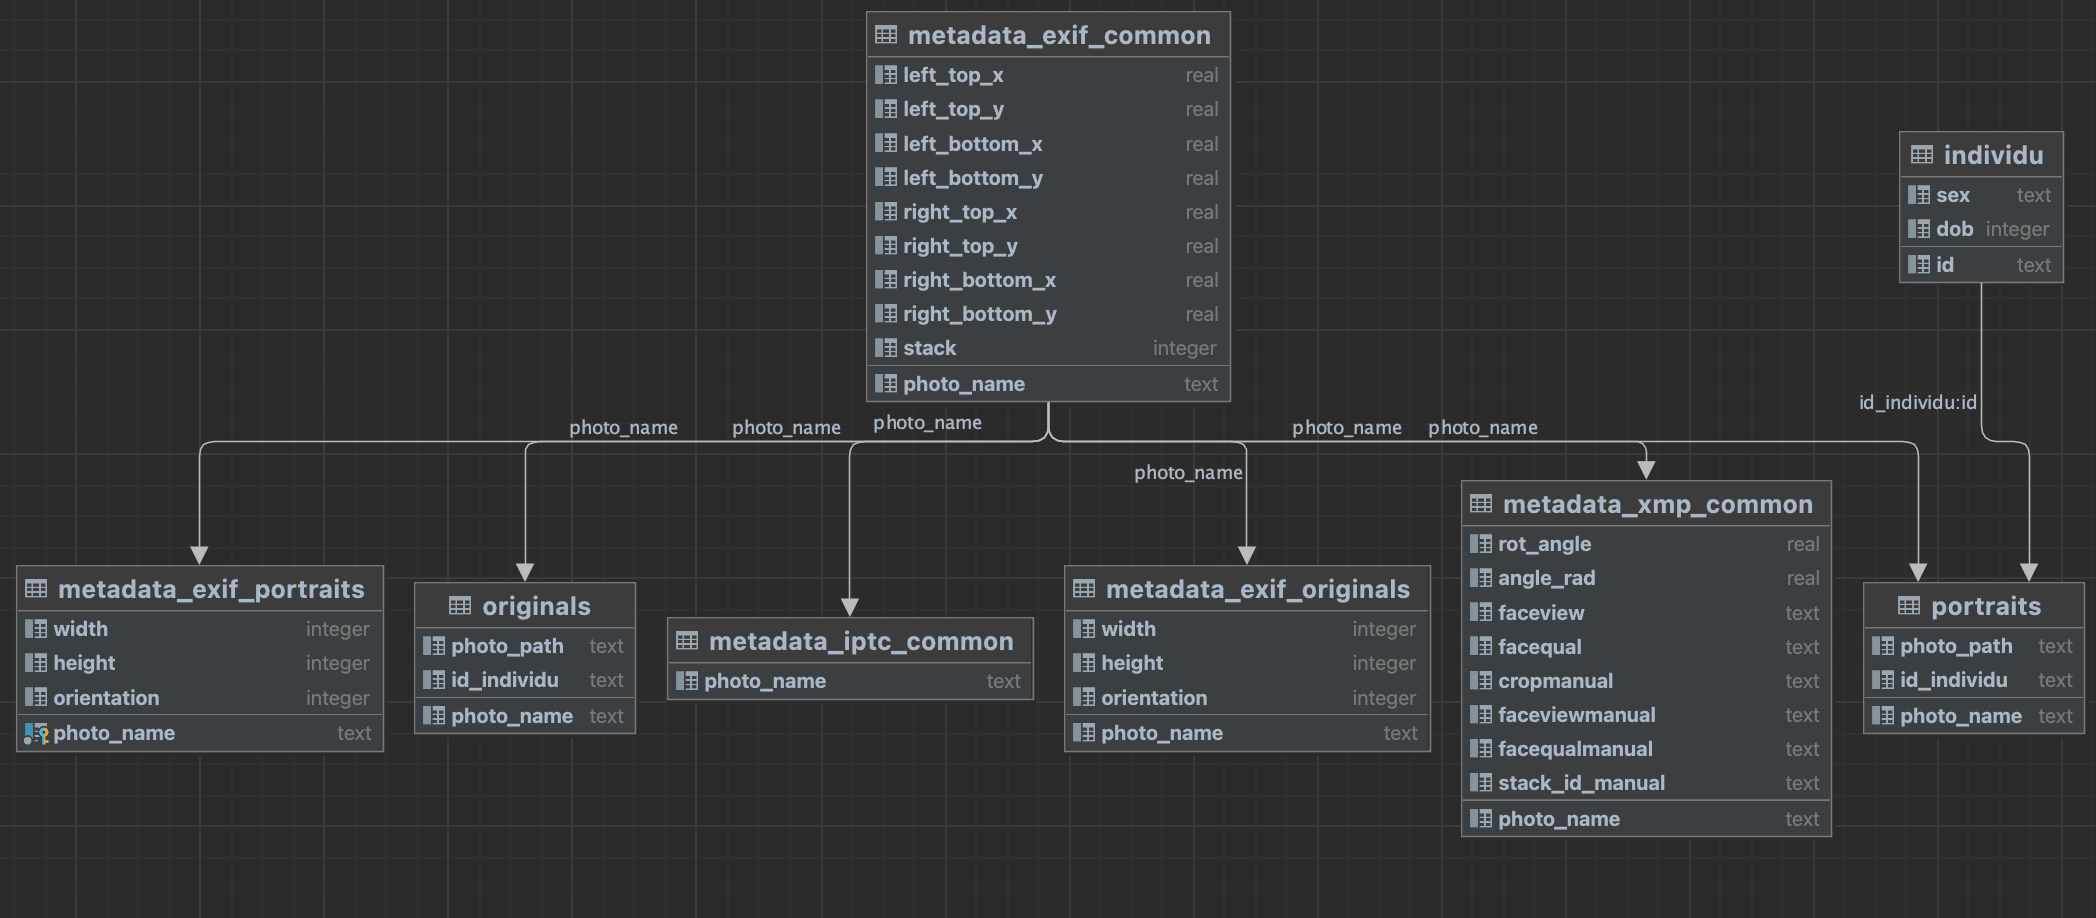
\includegraphics[width=450pt]{imgs/qualité/cr8/sqlite_schema.png}
\end{center}

\subsection{Utilisation de \Gls{docker}}
Pour améliorer la portabilité de tous les scripts, j'ai mis en place Docker ainsi que Docker Compose. Docker est un logiciel basé sur la virtualisation (notion de conteneurs, isolés du système hôte), qui permet de lancer un script avec son environnement (système d'exploitation et dépendances) "figé", de sorte qu'il fonctionne de manière reproductible dans le temps et partout.\\

En effet, lorsqu'on doit installer un environnent de travail \gls{tensorflow}, il y a besoin de respecter une matrice de compatibilité des dépendances, ce qui peut s'avérer complexe avec les évolutions des différentes librairies dans le temps. De plus, l'interfaçage avec les drivers de cartes graphiques (GPU) ajoute une couche de complexité dans cette mise en place. 

Dans la logique \Gls{docker}, on peut écrire des Dockerfile afin de construire des images étendues personnalisées en partant d'image de base existantes (qui peuvent elles même être des images étendues).

On peut également utiliser Docker Compose pour orchestrer les lancements des conteneurs basé sur les images. Ceci est utile pour stocker les configurations plutôt que d'utiliser les nombreux paramètres en lignes de commande.

Voici des exemples de mes Dockerfile et docker-compose.yml : \\

Dans le Dockerfile, nous précisions l'image de base (un OS ou, ici, un OS déjà étendu avec une version spécifique de Python). Ensuite nous construisons l'image étendue, en y copiant les scripts locaux et en installant les dépendances enregistrées dans un fichier requirements.txt (qui est le standard pour le gestionnaire de dépendances python pip). Enfin la commande ENTRYPOINT indique le point de départ de l'application, et CMD les paramètres par défaut, qui sont pour leur part surchargeables.
\begin{center}
    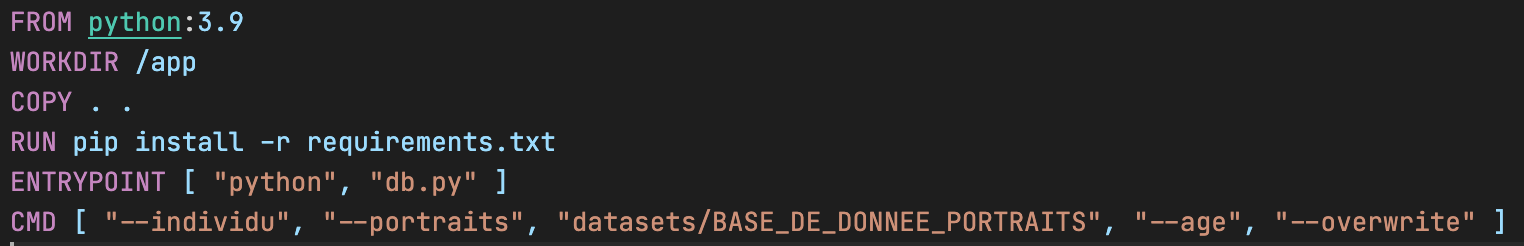
\includegraphics[width=450pt]{imgs/qualité/cr9/dockerfile.png}
\end{center}

Dans docker-compose.yml, nous pouvons orchestrer le lancement de plusieurs conteneurs Docker issus de Dockerfile pour qu'ils soient dépendants les uns des autres (les scripts d'IA nécessitants la base de donnée par exemple) ou simplement les lancer individuellement. Cela permet également de décrire pour les services, les volumes (bind mounts) directement dans un fichier de configuration, plutôt que comme paramètres de la commande Docker. Sans ces volumes montés, les données produites par les scripts ne seraient pas persistantes, car les conteneurs lancés avec Docker sont éphémères.
\begin{center}
    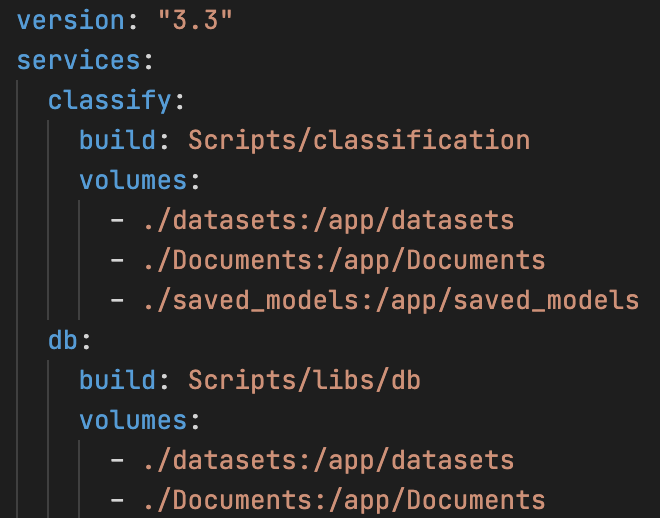
\includegraphics[width=200pt]{imgs/qualité/cr9/compose.png}
\end{center}

Voici un exemple de build des images, et de run de l'image de la base de donnée (le service db). Comme le docker-compose indique l'utilisation de bind mounts, le répertoire /app/Documents/Metadata/metadata.sqlite dans le container n'est autre que le fichier [projet]/Documents/Metadata/metadata.sqlite sur le système hôte (persistant).
\begin{center}
    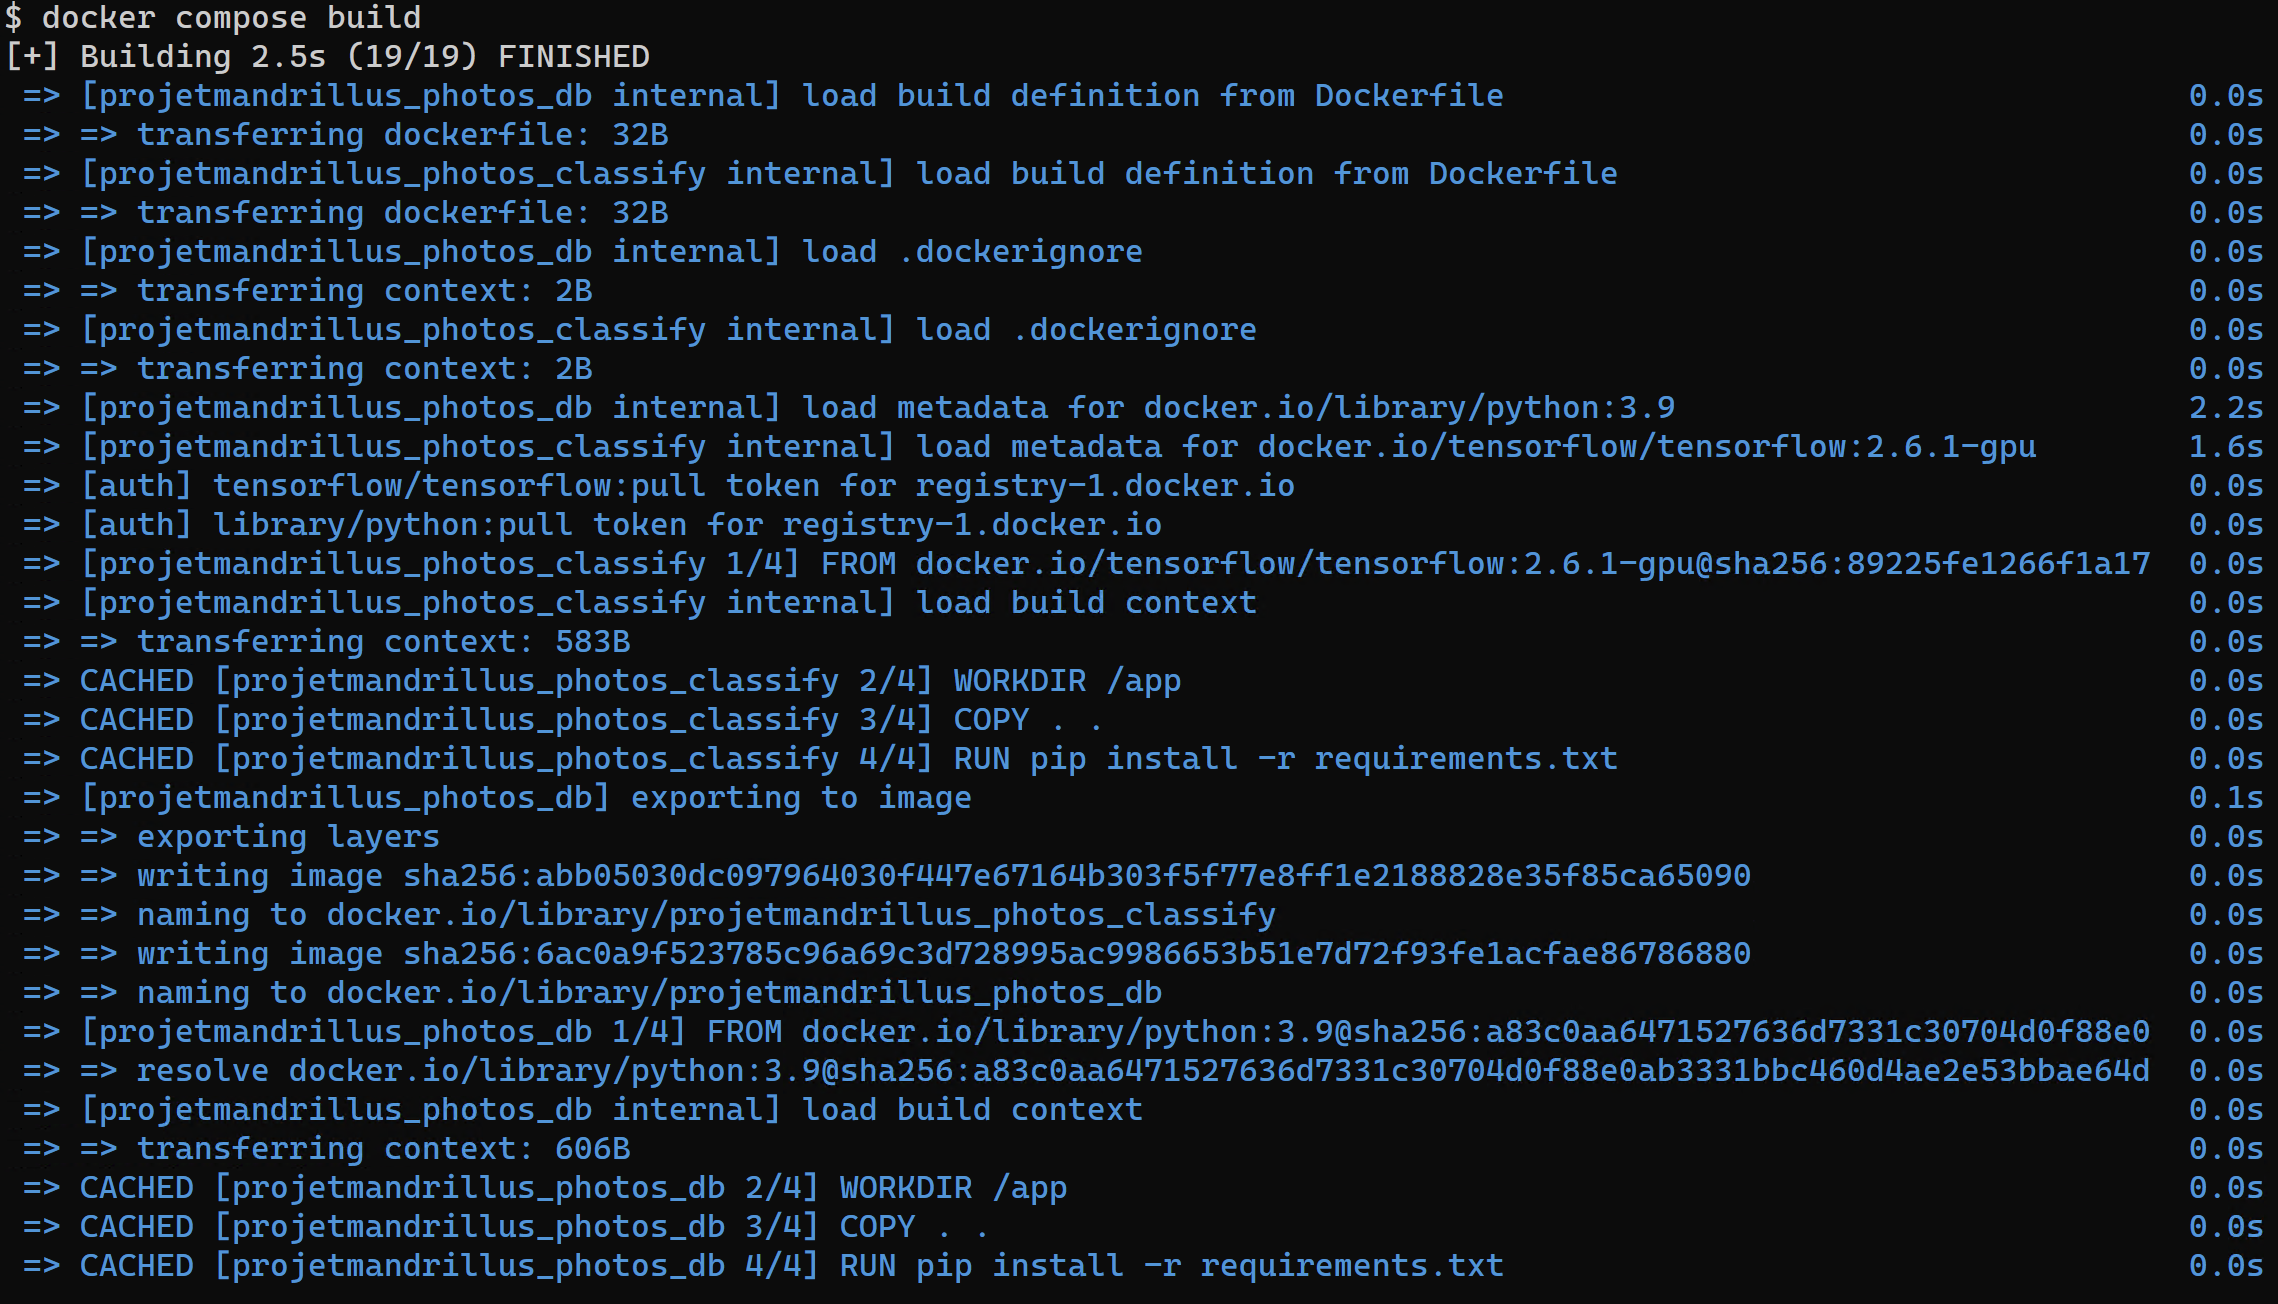
\includegraphics[width=450pt]{imgs/qualité/cr9/build.png}
    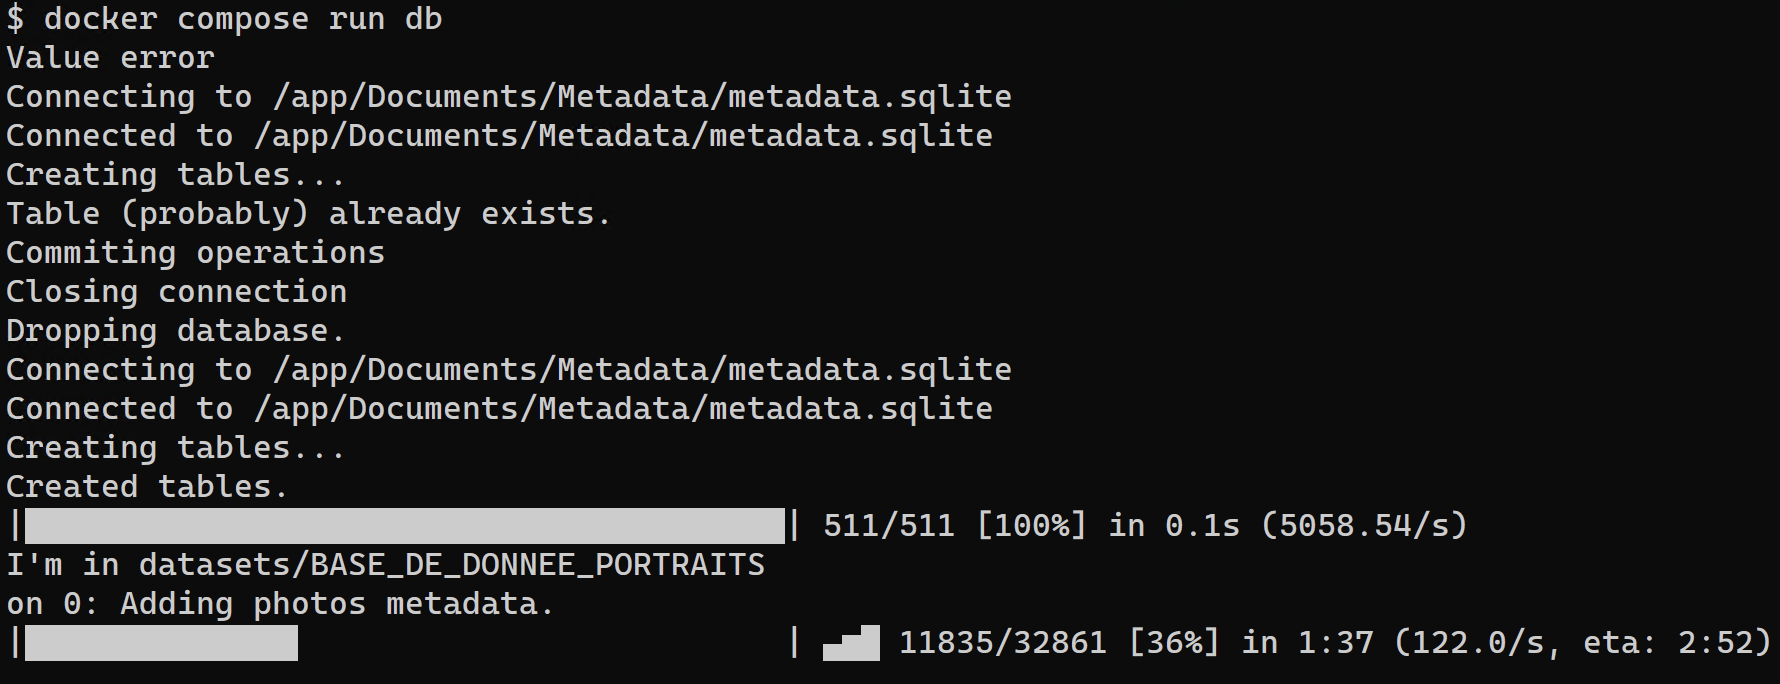
\includegraphics[width=450pt]{imgs/qualité/cr9/run.png}
\end{center}

\subsection{Modifications des keywords}
Les keywords sont un champs de métadonnées IPTC/\gls{XMP}, c'est-à-dire de métadonnées de photographies (jpeg), lues notamment par Adobe Lightroom. A mon arrivée, le champs Keywords contenait une liste d'éléments comme 1FaceQual3 pour indiquer une photo de bonne qualité, 1FaceQual2 pour une photo de qualité un peu moindre, ainsi que 1FaceView pour indiquer si le mandrill est de face, etc. \\ 

Seulement ce n'était pas très robuste à la lecture, si un des champs (comme la qualité) venait à manquer, puisque la liste était ensuite dans le mauvais ordre. On a donc changé vers début mai l'inscription de la manière suivante :
\begin{itemize}
    \item 1FaceQual0 devient FaceQual:0
    \item 1FaceQual1 devient FaceQual:1
    \item 1FaceQual2 devient FaceQual:2
    \item 1FaceQual3 devient FaceQual:3
    \item Le reste devient FaceQual:-1
\end{itemize}
De même pour tous les autres mots clés (FaceView pour n'en citer qu'un).

\subsection{Gridsearch}
La méthode de recherche gridsearch consiste à énumérer toutes les possibilités pour un certain nombre d'hyperparamètres en machine learning. Cela veut dire, lancer l'entraînement avec par exemple, un batchsize de 32, puis de 64, puis répéter le processus en changeant également le learning rate.
\begin{center}
    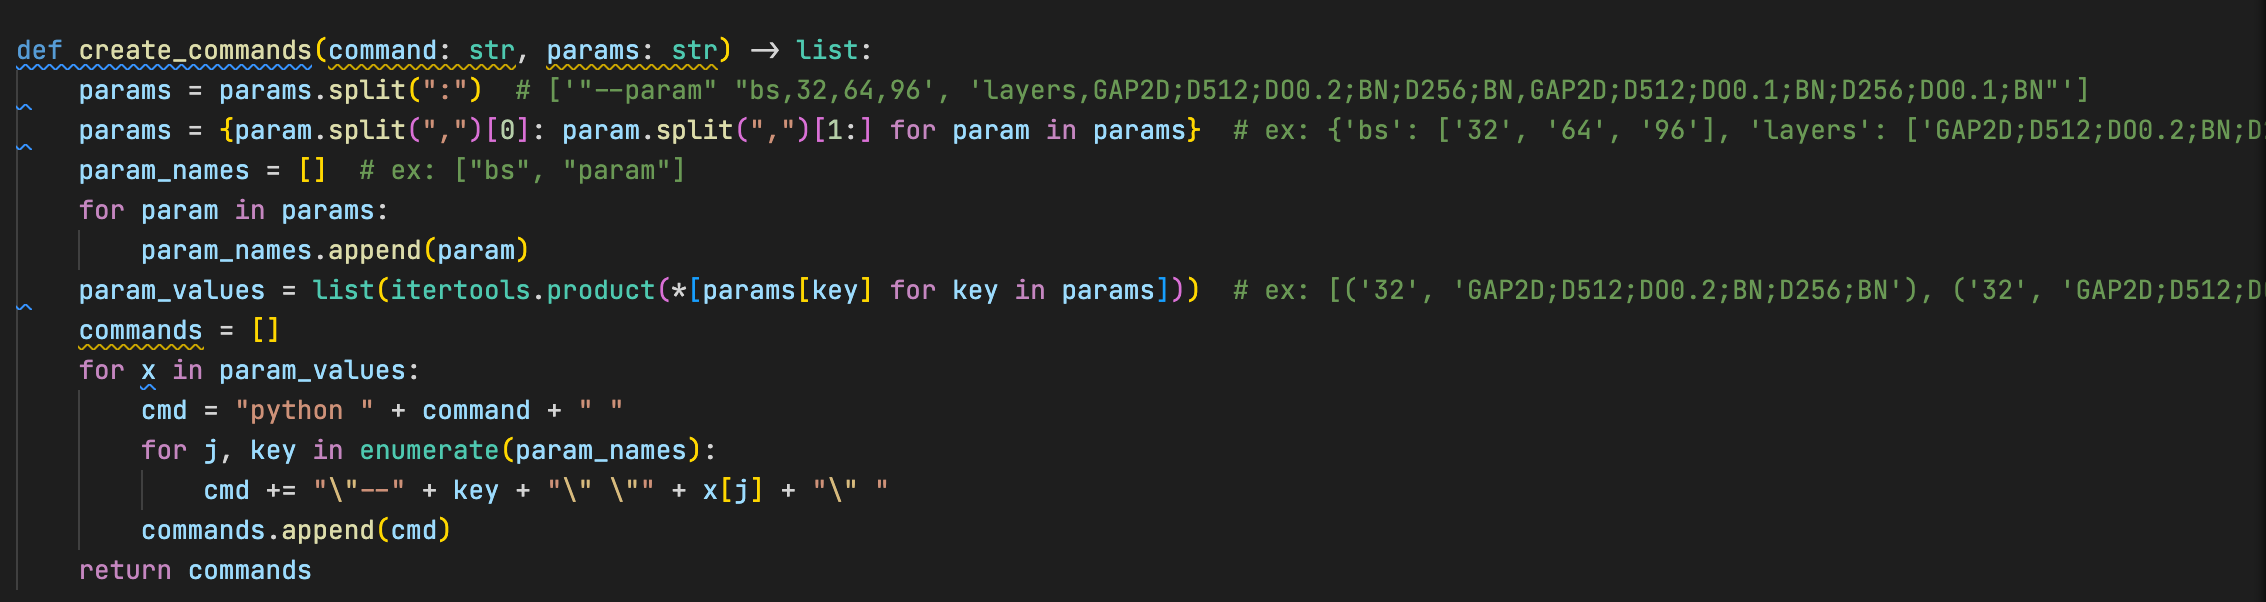
\includegraphics[width=450pt]{imgs/qualité/cr10/gridsearch.png}
    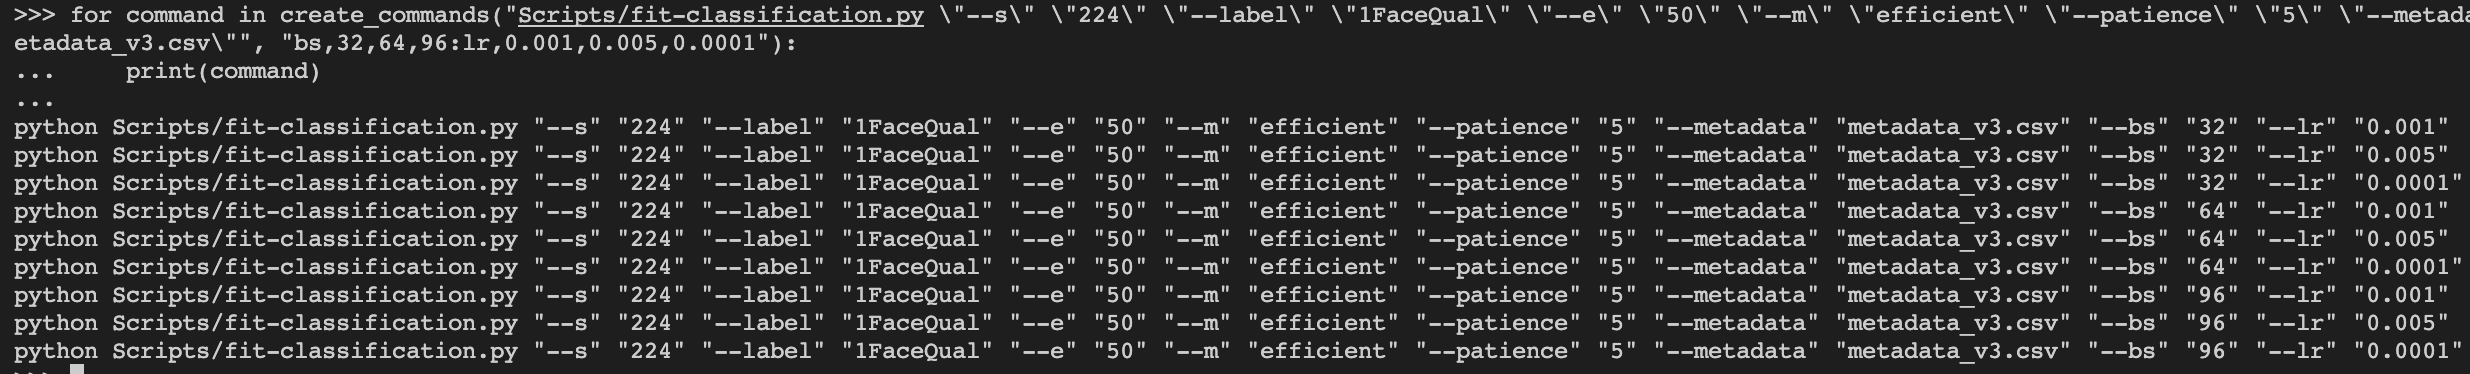
\includegraphics[width=450pt]{imgs/qualité/cr10/gridsearch2.png}
\end{center}
Comme on le voit ci-dessus : les commandes pour lancer les entraînements sont générés (et le script les lancent séquentiellement) en énumérant tous les hyperparamètres que l'on a spécifiés.